% Rank chips in Notes; \providecommand avoids duplicate-definition errors if already in main.tex.
\providecommand{\rankchip}[2]{\begingroup\setlength{\fboxsep}{1.2pt}\textcolor{black}{\colorbox[HTML]{#1}{\scriptsize\,#2\,}}\endgroup}
\begin{table*}[t]
    \centering
    \caption{\textbf{Main results on Llama-3.1-8B (accuracy, \%).}}
    \vspace{-2mm}
    \label{tab:main_results_llama}
    \footnotesize
    {\setlength{\tabcolsep}{1.85pt}%
     \setlength{\aboverulesep}{0pt}%
     \setlength{\belowrulesep}{0pt}%
     \setlength{\extrarowheight}{0pt}%
     \renewcommand{\arraystretch}{1.06}%
     \renewcommand{\tabularxcolumn}[1]{m{#1}}%
    \begin{tabularx}{\linewidth}{@{} >{\centering\arraybackslash}p{1.65cm} >{\centering\arraybackslash}m{1.28cm} !{\vrule width 0.4pt} >{\centering\arraybackslash}X >{\centering\arraybackslash}X >{\centering\arraybackslash}X >{\centering\arraybackslash}m{3.1em} >{\centering\arraybackslash}X >{\centering\arraybackslash}X >{\centering\arraybackslash}X >{\centering\arraybackslash}X >{\centering\arraybackslash}X >{\columncolor[HTML]{EAECEF}\centering\arraybackslash}m{3.1em} @{}}
    \toprule
    \multirow{2}{=}{\centering\textbf{Category}} & \multirow{2}{=}{\centering\textbf{Method}}
    & \multicolumn{4}{>{\cellcolor[HTML]{E3F2FD}}c!{\vrule width 1pt}}{\textbf{Quantitative Reasoning}}
    & \multicolumn{6}{>{\cellcolor[HTML]{E3F2FD}}c}{\textbf{Symbolic and Code}} \\
    &
    & {\small\textbf{GSM}} & {\small\textbf{MATH}} & {\small\textbf{DROP}} & \multicolumn{1}{>{\centering\arraybackslash}m{3.1em}!{\vrule width 1pt}}{\small\textbf{avg.}}
    & {\small\textbf{FOL}} & {\small\textbf{PW}} & {\small\textbf{BBH}} & {\small\textbf{HE}} & {\small\textbf{MBPP}} & \multicolumn{1}{>{\centering\arraybackslash}m{3.1em}}{\small\textbf{avg.}} \\
    \midrule
    Greedy & Vanilla & 79.0 & 58.2 & 6.2 & \multicolumn{1}{>{\centering\arraybackslash}m{3.1em}!{\vrule width 1pt}}{\cellcolor[HTML]{EAECEF}{53.9}} & 29.6 & 26.0 & 26.0 & 25.0 & \cellcolor[HTML]{FFD4D3}{55.2} & 33.0 \\
    \midrule
    \multirow{7}{=}{\centering Reasoning Paradigm}
    & CoT   & \cellcolor[HTML]{FFFCE0}{80.8} & \cellcolor[HTML]{FFD4D3}{64.2} & 1.7 & \multicolumn{1}{>{\centering\arraybackslash}m{3.1em}!{\vrule width 1pt}}{\cellcolor[HTML]{EAECEF}{55.5}} & 4.9 & 24.5 & \cellcolor[HTML]{FCE4D5}{70.0} & 25.0 & \cellcolor[HTML]{FCE4D5}{51.6} & 31.2 \\
    & PS    & 71.2 & 40.0 & 1.4 & \multicolumn{1}{>{\centering\arraybackslash}m{3.1em}!{\vrule width 1pt}}{\cellcolor[HTML]{EAECEF}{43.4}} & 4.9 & 15.2 & \cellcolor[HTML]{FFFCE0}{55.0} & 10.0 & 22.0 & 17.6 \\
    & SR    & 75.8 & 44.8 & \cellcolor[HTML]{FFFCE0}{15.6} & \multicolumn{1}{>{\centering\arraybackslash}m{3.1em}!{\vrule width 1pt}}{\cellcolor[HTML]{EAECEF}{50.4}} & 32.5 & 31.0 & 46.0 & 25.0 & 36.4 & 32.9 \\
    & SC    & \cellcolor[HTML]{FFD4D3}{83.6} & 54.0 & 1.6 & \multicolumn{1}{>{\centering\arraybackslash}m{3.1em}!{\vrule width 1pt}}{\cellcolor[HTML]{EAECEF}{53.2}} & 16.8 & 28.5 & 52.0 & 10.0 & 35.2 & 27.3 \\
    & BoN   & \cellcolor[HTML]{FFD4D3}{83.6} & 54.0 & 1.6 & \multicolumn{1}{>{\centering\arraybackslash}m{3.1em}!{\vrule width 1pt}}{\cellcolor[HTML]{EAECEF}{53.2}} & 16.8 & 28.5 & 52.0 & 10.0 & 35.2 & 27.3 \\
    & CB    & 48.0 & 36.5 & \cellcolor[HTML]{FCE4D5}{19.8} & \multicolumn{1}{>{\centering\arraybackslash}m{3.1em}!{\vrule width 1pt}}{\cellcolor[HTML]{EAECEF}{37.1}} & \cellcolor[HTML]{FFFCE0}{40.4} & \cellcolor[HTML]{FFFCE0}{35.8} & 34.0 & \cellcolor[HTML]{FFFCE0}{30.0} & \cellcolor[HTML]{FFFCE0}{49.2} & 38.6 \\
    & MCTS  & 55.2 & 33.5 & 13.2 & \multicolumn{1}{>{\centering\arraybackslash}m{3.1em}!{\vrule width 1pt}}{\cellcolor[HTML]{EAECEF}{37.5}} & 36.0 & 31.5 & 30.0 & \cellcolor[HTML]{FCE4D5}{35.0} & \cellcolor[HTML]{FFFCE0}{49.2} & 36.7 \\
    \midrule
    \multirow{3}{=}{\centering Memory-Oriented}
    & H2O    & 79.8 & 59.2 & 2.4 & \multicolumn{1}{>{\centering\arraybackslash}m{3.1em}!{\vrule width 1pt}}{\cellcolor[HTML]{EAECEF}{53.6}} & 6.4 & 27.8 & 48.0 & 10.0 & 42.0 & 26.3 \\
    & SNAP   & 80.4 & \cellcolor[HTML]{FCE4D5}{60.2} & 2.3 & \multicolumn{1}{>{\centering\arraybackslash}m{3.1em}!{\vrule width 1pt}}{\cellcolor[HTML]{EAECEF}{54.1}} & 8.4 & 26.2 & \cellcolor[HTML]{FFFCE0}{55.0} & 15.0 & 41.2 & 27.3 \\
    & STREAM & 70.4 & 44.2 & 1.3 & \multicolumn{1}{>{\centering\arraybackslash}m{3.1em}!{\vrule width 1pt}}{\cellcolor[HTML]{EAECEF}{44.4}} & 1.5 & 31.8 & 1.0 & 0.0 & 5.6 & 13.0 \\
    \midrule
    Latent & COCO & \cellcolor[HTML]{FCE4D5}{81.4} & \cellcolor[HTML]{FFFCE0}{60.0} & 3.7 & \multicolumn{1}{>{\centering\arraybackslash}m{3.1em}!{\vrule width 1pt}}{\cellcolor[HTML]{EAECEF}{54.8}} & \cellcolor[HTML]{FFD4D3}{45.3} & \cellcolor[HTML]{FCE4D5}{45.2} & 51.0 & 20.0 & 47.2 & 42.5 \\
    \midrule
    RL-Based & GRPO & 0.0 & 0.5 & 0.3 & \multicolumn{1}{>{\centering\arraybackslash}m{3.1em}!{\vrule width 1pt}}{\cellcolor[HTML]{EAECEF}{0.2}} & 2.0 & 2.2 & 7.0 & 0.0 & 0.0 & 1.8 \\
    \midrule
    Ours & \textbf{SoT} & \cellcolor[HTML]{FFD4D3}{\textbf{83.6}} & \textbf{54.8} & \cellcolor[HTML]{FFD4D3}{\textbf{38.9}} & \multicolumn{1}{>{\centering\arraybackslash}m{3.1em}!{\vrule width 1pt}}{\cellcolor[HTML]{EAECEF}{\underline{\textbf{62.8}}}} & \cellcolor[HTML]{FCE4D5}{\textbf{43.4}} & \cellcolor[HTML]{FFD4D3}{\textbf{60.2}} & \cellcolor[HTML]{FFD4D3}{\textbf{77.0}} & \cellcolor[HTML]{FFD4D3}{\textbf{48.8}} & \cellcolor[HTML]{FFFCE0}{\textbf{49.2}} & \underline{\textbf{54.5}} \\
    \midrule
    \end{tabularx}\par\addvspace{0.35ex}
    \begin{tabularx}{\linewidth}{@{} >{\centering\arraybackslash}p{1.65cm} >{\centering\arraybackslash}m{1.28cm} !{\vrule width 0.4pt} >{\centering\arraybackslash}X >{\centering\arraybackslash}X >{\centering\arraybackslash}X >{\centering\arraybackslash}X >{\centering\arraybackslash}X >{\centering\arraybackslash}m{3.1em} >{\centering\arraybackslash}X >{\centering\arraybackslash}X >{\centering\arraybackslash}X >{\columncolor[HTML]{EAECEF}\centering\arraybackslash}m{3.1em} @{}}
    \multirow{2}{=}{\centering\textbf{Category}} & \multirow{2}{=}{\centering\textbf{Method}}
    & \multicolumn{6}{>{\cellcolor[HTML]{E3F2FD}}c!{\vrule width 1pt}}{\textbf{General Understanding}}
    & \multicolumn{4}{>{\cellcolor[HTML]{E3F2FD}}c}{\textbf{Long-Context Reasoning}} \\
    &
    & {\small\textbf{CSQA}} & {\small\textbf{StrQA}} & {\small\textbf{BoolQ}} & {\small\textbf{MMLU}} & {\small\textbf{RACE}} & \multicolumn{1}{>{\centering\arraybackslash}m{3.1em}!{\vrule width 1pt}}{\small\textbf{avg.}}
    & {\small\textbf{HQA}} & {\small\textbf{NarQA}} & {\small\textbf{LB}} & \multicolumn{1}{>{\centering\arraybackslash}m{3.1em}}{\small\textbf{avg.}} \\
    \midrule
    Greedy & Vanilla & \cellcolor[HTML]{FFFCE0}{48.0} & \cellcolor[HTML]{FCE4D5}{68.8} & 59.2 & 45.6 & 50.7 & \multicolumn{1}{>{\centering\arraybackslash}m{3.1em}!{\vrule width 1pt}}{\cellcolor[HTML]{EAECEF}{54.2}} & 7.0 & 20.1 & \cellcolor[HTML]{FFFCE0}{32.7} & 16.2 \\
    \midrule
    \multirow{7}{=}{\centering Reasoning Paradigm}
    & CoT   & 32.8 & 31.5 & 37.2 & 34.0 & 50.3 & \multicolumn{1}{>{\centering\arraybackslash}m{3.1em}!{\vrule width 1pt}}{\cellcolor[HTML]{EAECEF}{36.3}} & 2.0 & 4.5 & 26.9 & 7.1 \\
    & PS    & 30.5 & 18.2 & 21.5 & 31.2 & 42.0 & \multicolumn{1}{>{\centering\arraybackslash}m{3.1em}!{\vrule width 1pt}}{\cellcolor[HTML]{EAECEF}{28.1}} & 1.7 & 3.0 & 20.4 & 5.3 \\
    & SR    & \cellcolor[HTML]{FCE4D5}{57.0} & 64.0 & \cellcolor[HTML]{FFFCE0}{72.2} & \cellcolor[HTML]{FCE4D5}{62.4} & \cellcolor[HTML]{FCE4D5}{62.7} & \multicolumn{1}{>{\centering\arraybackslash}m{3.1em}!{\vrule width 1pt}}{\cellcolor[HTML]{EAECEF}{63.6}} & \cellcolor[HTML]{FCE4D5}{17.9} & 21.7 & 25.5 & 20.6 \\
    & SC    & 28.5 & 34.5 & 43.2 & 31.0 & 45.7 & \multicolumn{1}{>{\centering\arraybackslash}m{3.1em}!{\vrule width 1pt}}{\cellcolor[HTML]{EAECEF}{35.8}} & 1.9 & 4.3 & 25.8 & 6.8 \\
    & BoN   & 28.5 & 34.5 & 43.2 & 31.0 & 45.7 & \multicolumn{1}{>{\centering\arraybackslash}m{3.1em}!{\vrule width 1pt}}{\cellcolor[HTML]{EAECEF}{35.8}} & 1.9 & 4.3 & 25.8 & 6.8 \\
    & CB    & 46.0 & \cellcolor[HTML]{FFD4D3}{71.5} & \cellcolor[HTML]{FFD4D3}{82.2} & \cellcolor[HTML]{FFFCE0}{51.2} & \cellcolor[HTML]{FFFCE0}{56.0} & \multicolumn{1}{>{\centering\arraybackslash}m{3.1em}!{\vrule width 1pt}}{\cellcolor[HTML]{EAECEF}{61.1}} & \cellcolor[HTML]{FFFCE0}{15.5} & \cellcolor[HTML]{FCE4D5}{27.5} & 26.2 & 21.8 \\
    & MCTS  & 42.0 & 65.5 & \cellcolor[HTML]{FFD4D3}{82.2} & 46.4 & 49.7 & \multicolumn{1}{>{\centering\arraybackslash}m{3.1em}!{\vrule width 1pt}}{\cellcolor[HTML]{EAECEF}{57.0}} & 13.5 & \cellcolor[HTML]{FFFCE0}{27.1} & 27.8 & 21.0 \\
    \midrule
    \multirow{3}{=}{\centering Memory-Oriented}
    & H2O    & 33.5 & 30.8 & 39.2 & 35.0 & 19.7 & \multicolumn{1}{>{\centering\arraybackslash}m{3.1em}!{\vrule width 1pt}}{\cellcolor[HTML]{EAECEF}{32.4}} & 2.0 & 2.0 & 0.0 & 1.7 \\
    & SNAP   & 33.5 & 31.0 & 38.5 & 34.6 & 16.7 & \multicolumn{1}{>{\centering\arraybackslash}m{3.1em}!{\vrule width 1pt}}{\cellcolor[HTML]{EAECEF}{31.8}} & 2.0 & 2.0 & 0.0 & 1.7 \\
    & STREAM & 34.8 & 26.2 & 38.8 & 22.4 & 0.0 & \multicolumn{1}{>{\centering\arraybackslash}m{3.1em}!{\vrule width 1pt}}{\cellcolor[HTML]{EAECEF}{25.6}} & 2.5 & 0.0 & 0.0 & 1.1 \\
    \midrule
    Latent & COCO & 40.5 & 63.5 & 70.0 & 42.8 & 43.3 & \multicolumn{1}{>{\centering\arraybackslash}m{3.1em}!{\vrule width 1pt}}{\cellcolor[HTML]{EAECEF}{52.0}} & 4.4 & 10.8 & \cellcolor[HTML]{FCE4D5}{34.6} & 11.9 \\
    \midrule
    RL-Based & GRPO & 10.5 & 3.8 & 9.8 & 8.2 & 12.0 & \multicolumn{1}{>{\centering\arraybackslash}m{3.1em}!{\vrule width 1pt}}{\cellcolor[HTML]{EAECEF}{8.7}} & 0.6 & 1.1 & 5.3 & 1.6 \\
    \midrule
    Ours & \textbf{SoT} & \cellcolor[HTML]{FFD4D3}{\textbf{71.0}} & \cellcolor[HTML]{FFFCE0}{\textbf{67.2}} & \cellcolor[HTML]{FCE4D5}{\textbf{80.0}} & \cellcolor[HTML]{FFD4D3}{\textbf{64.6}} & \cellcolor[HTML]{FFD4D3}{\textbf{75.7}} & \multicolumn{1}{>{\centering\arraybackslash}m{3.1em}!{\vrule width 1pt}}{\cellcolor[HTML]{EAECEF}{\underline{\textbf{71.1}}}} & \cellcolor[HTML]{FFD4D3}{\textbf{25.7}} & \cellcolor[HTML]{FFD4D3}{\textbf{39.4}} & \cellcolor[HTML]{FFD4D3}{\textbf{38.3}} & \underline{\textbf{33.0}} \\
    \bottomrule
    \end{tabularx}%
    }
    \vspace{0.35ex}
    \noindent\begin{minipage}{\linewidth}
        \footnotesize
        \textbf{Note.} Other model results are reported in Table~\ref{tab:app_main_qwen}, ~\ref{tab:app_main_mixtral}.
        Cells colored with rankings as \rankchip{FFD4D3}{1st}, \rankchip{FCE4D5}{2nd}, and \rankchip{FFFCE0}{3rd}.
    \end{minipage}
    \vspace{-7mm}
    \end{table*}
    
    \section{Experiments}
    \label{sec:exp}
    \vspace{-2mm}
    % We evaluate State of Thought from two complementary perspectives: \emph{generalization} and \emph{efficiency}, to test whether an endogenous state-driven reasoning paradigm can remain effective across heterogeneous reasoning regimes without relying on a fixed externally prescribed reasoning template.
    
    \subsection{Experimental Setup}
    \label{sec:setup}
    
    \paragraph{Backbone models.}
    We evaluate SoT on three frozen \emph{LLMs} with different scales and architectures (Llama-3.1-8B \citep{grattafiori2024llama3}, Qwen2.5-14B \citep{yang2024qwen25}, and Mixtral-8x7B \citep{jiang2024mixtral})
    and transfer to the frozen \emph{Vision Language Model (VLM)} (Qwen3-VL-8B \citep{qwen2025qwen3vl8b}). Full details are deferred to Appendix~\ref{app:model_protocol}.
    
    \paragraph{Tasks and evaluation domains.}
    For \emph{LLMs}, we organize evaluation into \emph{four reasoning domains} comprising \emph{16 benchmarks}.
    \textbf{Quantitative Reasoning} (QS) includes GSM8K (GSM) \citep{cobbe2021gsm8k}, MATH \citep{hendrycks2021measuring}, and DROP \citep{dua2019drop}.
    \textbf{General Understanding} (GU) includes CommonsenseQA (CSQA) \citep{talmor2019commonsenseqa}, StrategyQA (StrQA) \citep{geva2021did}, BoolQ \citep{clark2019boolq}, MMLU \citep{hendrycks2021measuringmassive}, and RACE \citep{lai2017race}.
    \textbf{Symbolic and Code} (S\&C) includes FOLIO (FOL) \citep{han2024folio}, ProofWriter (PW) \citep{tafjord2021proofwriter}, BBH-Temporal (BBH) \citep{srivastava2023beyond}, HumanEval (HE) \citep{chen2021evaluating}, and MBPP \citep{austin2021program}.
    \textbf{Long-Context Reasoning} (LCR) includes HotpotQA (HQA) \citep{yang2018hotpotqa}, NarrativeQA (NarQA) \citep{kocisky2018narrativeqa}, and LongBench MultiFieldQA (LB) \citep{bai2024longbench}.
    For \emph{VLM} transfer, we evaluate \emph{4 benchmarks}: Beans-M \citep{makerere2020beans}, Fashion-MNIST (F-MNIST) \citep{xiao2017fashion}, DocVQA \citep{mathew2021docvqa}, and InfographicVQA (InfoVQA) \citep{mathew2022infographicvqa}.
    Full details are deferred to Appendix~\ref{app:dataset_setup}.
    
    \paragraph{Baselines.}
    We compare SoT against \emph{5 baseline families}. 
    \textbf{Greedy:} Vanilla. 
    \textbf{Reasoning paradigm:} Chain-of-Thought (CoT) \citep{wei2022chain}, Plan-and-Solve (PS) \citep{wang2023plan}, Self-Refine (SR) \citep{madaan2023self} with externally scripted programs, and Self-Consistency (SC) \citep{wang2023selfconsistency}, Best-of-N (BoN) \citep{snell2024scaling}, Constrained Beam (CB) \citep{hokamp2017lexically}, Monte Carlo Tree Search (MCTS) \citep{xie2024mcts} with sampling or search methods.
    \textbf{Memory-oriented methods:} H$_2$O (H2O) \citep{zhang2023h2o}, SnapKV (SNAP) \citep{li2024snapkv}, and StreamingLLM (STREAM) \citep{xiao2023streamingllm}. 
    \textbf{Latent reasoning:} COCONUT (COCO) \citep{hao2025training}. 
    \textbf{RL-based reasoning:} GRPO \citep{shao2024deepseekmath}. 
    All trainable baselines share the same training data as SoT. Full details are deferred to Appendix~\ref{app:baseline_methods} and ~\ref{app:hyperparameters}.
    
\begin{table*}[t]
    \centering
    \vspace{-2mm}
    % --- 左侧约 0.8\textwidth；右侧图约 0.19\textwidth（表/图 ≈ 4:1，避免表身溢出压到图） ---
    \begin{minipage}[b]{0.75\textwidth}
        \centering
        % \captionsetup{skip=10pt}%
        \captionof{table}{\textbf{Efficiency comparison on Llama-3.1-8B.}} 
        \label{tab:efficiency}
        \vspace{-2mm}
        \footnotesize
        \begingroup
        \setlength{\tabcolsep}{0.80pt}%
        \setlength{\aboverulesep}{0pt}%
        \setlength{\belowrulesep}{0pt}%
        \setlength{\extrarowheight}{0pt}%
        \renewcommand{\arraystretch}{1.1}%
        \begin{tabular}{@{}
            >{\centering\arraybackslash}p{1.32cm}
            >{\centering\arraybackslash}m{3.35em}
            !{\vrule width 0.4pt}
            >{\centering\arraybackslash}m{3.05em}
            >{\centering\arraybackslash}m{3.05em}
            !{\vrule width 1pt}
            >{\centering\arraybackslash}m{3.05em}
            >{\centering\arraybackslash}m{3.05em}
            !{\vrule width 1pt}
            >{\centering\arraybackslash}m{3.05em}
            >{\centering\arraybackslash}m{3.05em}
            !{\vrule width 1pt}
            >{\centering\arraybackslash}m{3.05em}
            >{\centering\arraybackslash}m{3.05em}
            @{}}
        \toprule
        \multirow{2}{=}{\centering\textbf{Category}} & \multirow{2}{=}{\centering\textbf{Method}}
        & \multicolumn{2}{>{\cellcolor[HTML]{E3F2FD}}c!{\vrule width 1pt}}{\textbf{QS}}
        & \multicolumn{2}{>{\cellcolor[HTML]{E3F2FD}}c!{\vrule width 1pt}}{\textbf{S\&C}}
        & \multicolumn{2}{>{\cellcolor[HTML]{E3F2FD}}c!{\vrule width 1pt}}{\textbf{GU}}
        & \multicolumn{2}{>{\cellcolor[HTML]{E3F2FD}}c}{\textbf{LCR}} \\
        \cmidrule(lr){3-4}\cmidrule(lr){5-6}\cmidrule(lr){7-8}\cmidrule(lr){9-10}
        & & {\small\textbf{Tok.}} & {\small\textbf{Lat.}} & {\small\textbf{Tok.}} & {\small\textbf{Lat.}} & {\small\textbf{Tok.}} & {\small\textbf{Lat.}} & {\small\textbf{Tok.}} & {\small\textbf{Lat.}} \\
        \midrule
        \multirow{7}{=}{\centering Reasoning\\Paradigm}
        & CoT  & 271.6 & 17.5 & 369.8 & 27.5 & 212.9 & 12.8 & 198.1 & \cellcolor[HTML]{FFFCE0}{19.6} \\
        & PS   & 314.2 & 20.7 & 372.1 & 26.8 & 319.8 & 22.2 & 282.3 & 33.7 \\
        & SR   & 368.5 & 25.9 & 391.7 & 28.8 & 292.2 & 19.2 & 278.8 & 33.2 \\
        & SC   & 736.8 & 43.1 & 953.9 & 63.5 & 626.5 & 37.6 & 533.8 & 48.9 \\
        & BoN  & 736.8 & 43.2 & 953.9 & 63.5 & 626.5 & 36.9 & 533.8 & 49.0 \\
        & CB   & 423.9 & 22.0 & 363.9 & \cellcolor[HTML]{FCE4D5}{19.4} & 341.7 & 16.8 & 283.7 & \cellcolor[HTML]{FCE4D5}{19.5} \\
        & MCTS & 422.1 & 21.4 & 364.7 & \cellcolor[HTML]{FCE4D5}{19.4} & 335.2 & 16.5 & 286.6 & 20.5 \\
        \midrule
        \multirow{3}{=}{\centering Memory-\\Oriented}
        & H2O    & 226.0 & 16.7 & \cellcolor[HTML]{FFFCE0}{264.4} & 34.6 & 185.6 & 15.8 & \cellcolor[HTML]{FFFCE0}{155.8} & 21.5 \\
        & SNAP   & 226.0 & 16.6 & \cellcolor[HTML]{FFFCE0}{264.4} & 34.8 & 185.6 & 16.1 & \cellcolor[HTML]{FFFCE0}{155.8} & 20.9 \\
        & STR & \cellcolor[HTML]{FFD4D3}{92.6} & \cellcolor[HTML]{FFFCE0}{12.5} & \cellcolor[HTML]{FFD4D3}{64.2} & 24.0 & \cellcolor[HTML]{FFFCE0}{88.2} & \cellcolor[HTML]{FFFCE0}{9.8} & \cellcolor[HTML]{FFD4D3}{67.6} & \cellcolor[HTML]{FFD4D3}{10.3} \\
        \midrule
        Latent & COCO & \cellcolor[HTML]{FCE4D5}{171.5} & \cellcolor[HTML]{FCE4D5}{11.5} & \cellcolor[HTML]{FCE4D5}{214.6} & \cellcolor[HTML]{FFFCE0}{20.4} & \cellcolor[HTML]{FCE4D5}{87.2} & \cellcolor[HTML]{FCE4D5}{6.7} & \cellcolor[HTML]{FCE4D5}{131.5} & 30.3 \\
        \midrule
        RL-Based & GRPO\textsuperscript{\raisebox{-0.08ex}{\scriptsize\kern0.06em\textbf{+}}} & 73.1 & 7.5 & 69.7 & 7.1 & 71.4 & 7.5 & 76.2 & 26.9 \\
        \midrule
        Ours & \textbf{SoT} & \cellcolor[HTML]{FFFCE0}{\textbf{219.4}} & \cellcolor[HTML]{FFD4D3}{\textbf{5.8}} & \textbf{294.0} & \cellcolor[HTML]{FFD4D3}{\textbf{9.5}} & \cellcolor[HTML]{FFD4D3}{\textbf{64.0}} & \cellcolor[HTML]{FFD4D3}{\textbf{1.8}} & \textbf{181.6} & \textbf{22.0} \\
        \bottomrule
        \end{tabular}%
        \endgroup
        \par\vspace{1.15ex}
    \end{minipage}
    \hfill
    % --- 右侧占位图（窄栏，约占通栏宽度的 ~1/5） ---
    \begin{minipage}[b]{0.24\textwidth}
        \centering
        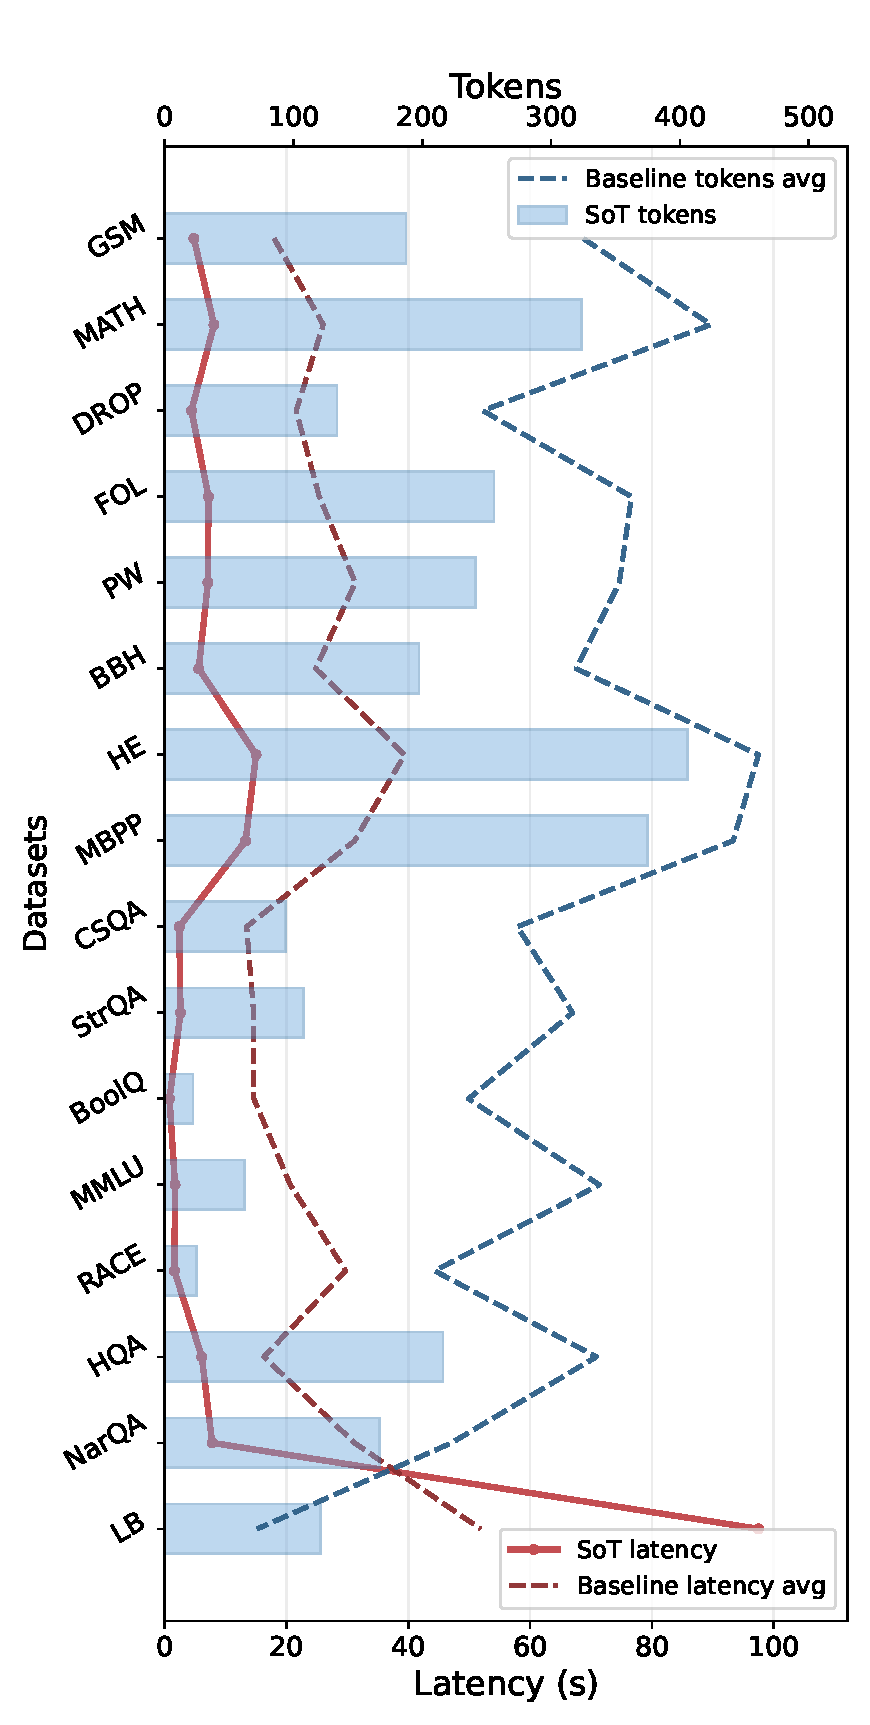
\includegraphics[width=0.92\textwidth]{figs/distribution_llama_tokens_latency.pdf}
        \vspace{-2mm}
        \captionof{figure}{\textbf{Distribution.}}
        \vspace{1mm}
        \label{fig:efficiency_datasets}
    \end{minipage}

    % --- 下方共享的 Notes ---
    %\par\vspace{1.05ex}\noindent
    \vspace{-1mm}
    \begin{minipage}{\textwidth}
        \footnotesize
        \noindent\textbf{Note.}
        Results of generated reasoning tokens (\textbf{Tok.}) and end-to-end latency (\textbf{Lat.}) are aggregated over four reasoning domains, with full breakdown in Table~\ref{tab:app_tok_llama}, ~\ref{tab:app_lat_llama}. Results of other models are in Table ~\ref{tab:app_tok_qwen}, ~\ref{tab:app_lat_qwen}, ~\ref{tab:app_tok_mixtral}, ~\ref{tab:app_lat_mixtral}.
    \end{minipage}
    \vspace{-4mm}
\end{table*}
    
    \begin{wrapfigure}{r}{0.55\columnwidth}
        \vspace{-3.0mm}
        \centering
        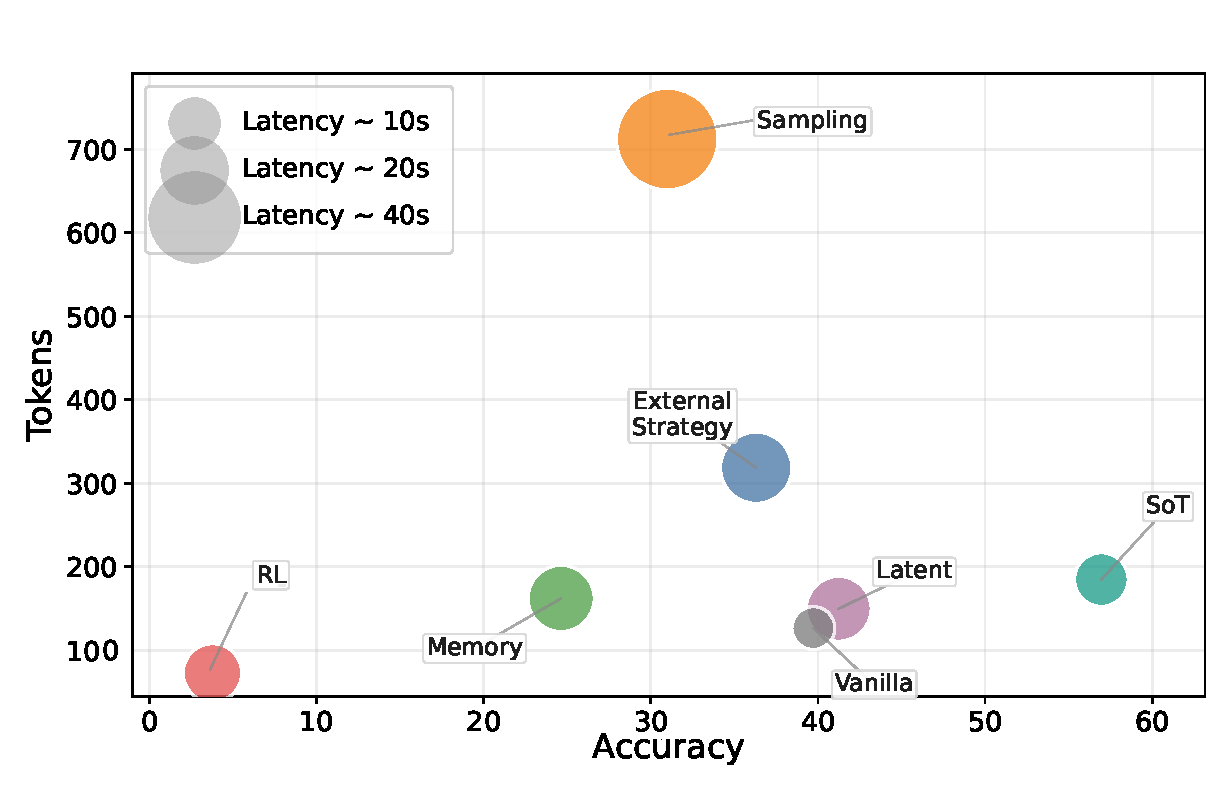
\includegraphics[width=0.53\textwidth]{figs/tradeoff_llama_grouped6.pdf}
        \vspace{-1mm}
        \caption{\textbf{Accuracy--efficiency trade-off} on Llama-3.1-8B with breakdown and other models in Figure~\ref{fig:app_tradeoff_all}.}
        \label{fig:acc_eff_tradeoff}
        \vspace{-12mm}
    \end{wrapfigure}
    
    \paragraph{Evaluation metrics.}
    We report task-standard accuracy metrics and efficiency cost. 
    \textbf{Exact Match (EM)} is used for GSM8K, MATH, RACE, MMLU, CommonsenseQA, FOL, BBH, ProofWriter, BoolQ, StrategyQA, Beans-M, Fashion-MNIST, DocVQA, and InfographicVQA. 
    \textbf{F1} is used for HotpotQA, DROP, NarrativeQA, and LongBench MultiFieldQA. 
    \textbf{Pass@1} is used for HumanEval and MBPP. 
    \textbf{Efficiency} is measured by generated tokens and end-to-end inference latency in H200.

    \vspace{-2mm}
    \subsection{Main Results}
    \label{sec:main_results}
    \vspace{-0.5mm}
    
    \paragraph{Overall performance.}
    Table~\ref{tab:main_results_llama} reports the main results on Llama-3.1-8B across four reasoning domains.
    SoT achieves the best domain-level average in all domains. 
    Compared with the strongest non-SoT baseline in each domain, it improves Quantitative Reasoning, Symbolic and Code, General Understanding, and Long-Context Reasoning by \(+7.3\), \(+12.0\), \(+7.5\), and \(+11.2\) points, corresponding to relative gains of \(13.2\%\), \(28.2\%\), \(11.8\%\), and \(51.4\%\). 
    It also obtains the best or tied-best result on 11 out of 16 datasets, with an average domain-level gain of \(9.5\) points over the strongest competing methods.
    This pattern suggests that reasoning gains need \emph{not} come primarily from prescribing a stronger external reasoning program or from scaling search over more trajectories. 
    A closed-loop controller driven by the model's own endogenous reasoning state can itself serve as an effective mechanism for improving test-time reasoning.
    We further demonstrate the stable performance gains of our method through quality sensitivity experiments on the training dataset in the Appendix~\ref{app:traj_quality}.

    \vspace{-2mm}
    \paragraph{Generalization.}
    A distinctive property of SoT is that the same controller can be applied across heterogeneous reasoning structures with stable performance.
    Compared with scripted reasoning, SoT avoids committing to a fixed external reasoning form; compared with sampling and search, it improves reasoning without relying mainly on broader trajectory expansion; compared with memory-oriented and latent reasoning baselines, it organizes historical evidence through the model's evolving endogenous state rather than generic context heuristics or hidden-space-only reasoning.
    Consistent gains across these regimes therefore indicate \emph{mechanism-level generalization}: SoT transfers as a reasoning principle, not merely as a benchmark-specific strategy.

    In general, these patterns suggest a more structural interpretation of the results.
    Within the family of externally prescribed token-chain reasoning methods, performance gains are typically obtained by strengthening scripts, increasing samples, or enlarging search.
    By contrast, SoT improves reasoning by changing the control variable itself, shifting from external token programs to endogenous state-conditioned evidence organization. This may explain why it can surpass strong token-chain baselines across heterogeneous regimes.
    Appendix~\ref{app:theory_policy_class} to ~\ref{app:theory_stop} provide in-depth theoretical analysis.

    \vspace{-3.0mm}

    \subsection{Efficiency and Trade-off}
    \label{sec:efficiency}
    \vspace{-0.5mm}
    
    Efficiency is central to inference-time reasoning because most performance gains come from expanding computation through longer trajectories, repeated sampling, or explicit search. Instead, SoT activates only the evidence context most suitable under the current endogenous state, so its advantage should appear not only in accuracy but also in efficiency.

    \vspace{-1.0mm}
    \paragraph{Efficiency.}
    Table~\ref{tab:efficiency} and Figure~\ref{fig:efficiency_datasets} report generated reasoning tokens and end-to-end latency on Llama-3.1-8B. Averaged over the four reasoning domains, SoT uses \(189.8\) tokens and \(9.8\)s latency, compared with \(532.7\) tokens and \(33.7\)s latency for sampling/search methods, reducing tokens by \(64.4\%\) and latency by \(70.8\%\). The saving is especially clear in QS, S\&C, and GU, where SoT attains strong accuracy with only \(5.8\)s, \(9.5\)s, and \(1.8\)s latency, respectively. Compared with memory-oriented methods, however, SoT is not merely a more aggressive compression rule: generic pruning can reduce tokens, but often sacrifices accuracy because it does not condition retained evidence on the current reasoning state. Thus, SoT improves efficiency by removing unnecessary computation while preserving the support needed for the next decision.

    \vspace{-1.0mm}
    \paragraph{Accuracy--efficiency trade-off.}
    Figure~\ref{fig:acc_eff_tradeoff} further shows that SoT moves the accuracy--efficiency frontier rather than simply trading accuracy for shorter outputs. It reaches the highest  accuracy while using far fewer tokens and lower latency than external strategies and sampling/search baselines. This pattern clarifies the core advantage of SoT: test-time compute is no longer spent on uniformly longer chains, larger candidate sets, or generic history retention, but is redirected toward state-conditioned evidence organization. The efficiency results therefore reinforce the main claim that endogenous reasoning state provides a better control signal for both reasoning quality and inference cost.
    
   \begin{table*}[t]
    \centering
    \vspace{-1mm}
    \caption{\textbf{Ablation results on Llama-3.1-8B,} with other models provided in Table~\ref{tab:app_ablation_qwen}, ~\ref{tab:app_ablation_mixtral}, ~\ref{tab:app_ablation_vlm}.}
    \vspace{-2mm}
    \label{tab:ablation}
    \footnotesize
    \setlength{\tabcolsep}{1.75pt}% 三组 acc/tok/lat 内侧略紧；竖线两旁用 \@kern 留空（避免贴线）
    \setlength{\aboverulesep}{0pt}%
    \setlength{\belowrulesep}{0pt}%
    \setlength{\extrarowheight}{0.75pt}% 微调行距，减轻彩色格上下“露白”（仍保持 rule sep 为 0）
    \renewcommand{\arraystretch}{1.0}%
    \begin{tabular}{l%
        @{\kern0.42em}!{\vrule width 0.4pt}@{\kern0.42em}%
        ccc%
        !{\vrule width 1pt}%
        ccc%
        !{\vrule width 1pt}%
        ccc%
        !{\vrule width 1pt}%
        ccc}
    \toprule
    \multirow{2}{*}{\textbf{Variant}} 
    & \multicolumn{3}{>{\columncolor[HTML]{E3F2FD}[\tabcolsep][\tabcolsep]}c!{\vrule width 1pt}}{\textbf{QS}} 
    & \multicolumn{3}{>{\columncolor[HTML]{E3F2FD}[\tabcolsep][\tabcolsep]}c!{\vrule width 1pt}}{\textbf{S\&C}} 
    & \multicolumn{3}{>{\columncolor[HTML]{E3F2FD}[\tabcolsep][\tabcolsep]}c!{\vrule width 1pt}}{\textbf{GU}} 
    & \multicolumn{3}{>{\columncolor[HTML]{E3F2FD}[\tabcolsep][\tabcolsep]}c}{\textbf{LCR}} \\
    \cmidrule(lr){2-4} \cmidrule(lr){5-7} \cmidrule(lr){8-10} \cmidrule(lr){11-13}
    & \textbf{acc.} & \textbf{tok.} & \textbf{lat.}
    & \textbf{acc.} & \textbf{tok.} & \textbf{lat.}
    & \textbf{acc.} & \textbf{tok.} & \textbf{lat.}
    & \textbf{acc.} & \textbf{tok.} & \textbf{lat.} \\
    \midrule
    Full SoT & 62.8 & 219.4 & 5.8 & 54.5 & 294.0 & 9.5 & 71.2 & 64.0 & 1.8 & 33.0 & 181.6 & 22.0 \\
    + Threshold Tuning & 62.8 & 219.4 & 5.8 & 54.3 & 294.0 & 9.5 & 71.2 & 64.0 & 1.8 & 31.8 & 229.0 & 22.0 \\
    \midrule
    % 使用简写省空间
    w/o Evid. Org. \(\mathcal{S}\) & 29.6 & 469.5 & 12.9 & 44.5 & 536.2 & 16.5 & \cellcolor[HTML]{EAECEF}{72.4} & 193.9 & 4.9 & 26.9 & 506.5 & \cellcolor[HTML]{EAECEF}{14.1} \\
    w/o Stopping \(\mathcal{T}\) & 60.6 & 1769.6 & 80.7 & \cellcolor[HTML]{EAECEF}{57.1} & 1705.1 & 110.3 & 70.2 & 4148.5 & 99.5 & 31.6 & 2937.4 & 157.3 \\
    w/o Geometry \(\delta_t\) & 42.5 & \cellcolor[HTML]{EAECEF}{68.6} & \cellcolor[HTML]{EAECEF}{3.3} & 46.4 & \cellcolor[HTML]{EAECEF}{48.0} & \cellcolor[HTML]{EAECEF}{2.9} & \cellcolor[HTML]{EAECEF}{73.0} & \cellcolor[HTML]{EAECEF}{25.4} & \cellcolor[HTML]{EAECEF}{0.9} & 24.5 & \cellcolor[HTML]{EAECEF}{47.2} & \cellcolor[HTML]{EAECEF}{2.2} \\
    w/o Dynamics \((v_t,c_t)\) & 57.0 & 1039.2 & 29.1 & 46.2 & 846.7 & 25.7 & 71.2 & 1272.3 & 33.7 & 31.6 & 1000.3 & 30.8 \\
    w/o Uncertainty \(H_t\) & 54.1 & 244.9 & 6.4 & 52.1 & \cellcolor[HTML]{EAECEF}{281.8} & \cellcolor[HTML]{EAECEF}{8.8} & \cellcolor[HTML]{EAECEF}{73.6} & \cellcolor[HTML]{EAECEF}{61.3} & 1.9 & 32.8 & 555.5 & \cellcolor[HTML]{EAECEF}{16.6} \\
    w/o Sent.-level Units & 54.1 & 244.9 & 7.2 & 52.1 & \cellcolor[HTML]{EAECEF}{281.8} & \cellcolor[HTML]{EAECEF}{8.8} & \cellcolor[HTML]{EAECEF}{73.6} & \cellcolor[HTML]{EAECEF}{61.3} & 1.9 & \cellcolor[HTML]{EAECEF}{35.1} & 224.1 & \cellcolor[HTML]{EAECEF}{11.9} \\
    \bottomrule
    \end{tabular}
    \vspace{-2mm}
\end{table*}

    \begin{table*}[t]
    \centering
    \captionsetup{skip=10pt}%
    \caption{\textbf{Transfer results on Qwen3-VL-8B.}}
    \label{tab:vlm_results}
    \vspace{-3mm}
    \footnotesize
    \begingroup
    % --- 参数保持不变 ---
    \setlength{\tabcolsep}{1.45pt}%
    \setlength{\aboverulesep}{0pt}%
    \setlength{\belowrulesep}{0pt}%
    \setlength{\extrarowheight}{0pt}%
    \renewcommand{\arraystretch}{1.06}%
    
    % 使用 makebox 强制表格相对于正文中心对齐，防止因微量溢出导致的向左偏移
    \makebox[\textwidth][c]{%
        \begin{tabular}{@{}
            >{\centering\arraybackslash}m{3.55em}!{\vrule width 0.4pt}
            *{3}{>{\centering\arraybackslash}m{3.05em}}
            !{\vrule width 1pt}
            *{3}{>{\centering\arraybackslash}m{3.05em}}
            !{\vrule width 1pt}
            *{3}{>{\centering\arraybackslash}m{3.05em}}
            !{\vrule width 1pt}
            *{3}{>{\centering\arraybackslash}m{3.05em}}
            @{}}
        \toprule
        \multirow{2}{=}{\textbf{Method}}
        & \multicolumn{3}{>{\cellcolor[HTML]{E3F2FD}}c!{\vrule width 1pt}}{\textbf{Beans-M}}
        & \multicolumn{3}{>{\cellcolor[HTML]{E3F2FD}}c!{\vrule width 1pt}}{\textbf{F-MNIST}}
        & \multicolumn{3}{>{\cellcolor[HTML]{E3F2FD}}c!{\vrule width 1pt}}{\textbf{DocVQA}}
        & \multicolumn{3}{>{\cellcolor[HTML]{E3F2FD}}c}{\textbf{InfoVQA}} \\
        \cmidrule(lr){2-4} \cmidrule(lr){5-7} \cmidrule(lr){8-10} \cmidrule(lr){11-13}
        & \textbf{acc.} & \textbf{tok.} & \textbf{lat.}
        & \textbf{acc.} & \textbf{tok.} & \textbf{lat.}
        & \textbf{acc.} & \textbf{tok.} & \textbf{lat.}
        & \textbf{acc.} & \textbf{tok.} & \textbf{lat.} \\
        \midrule
        CoT & \cellcolor[HTML]{FFFCE0}{80.8} & \cellcolor[HTML]{FFFCE0}{232.3} & \cellcolor[HTML]{FCE4D5}{29.9} & \cellcolor[HTML]{FCE4D5}{68.8} & \cellcolor[HTML]{FFFCE0}{225.7} & \cellcolor[HTML]{FCE4D5}{31.0} & \cellcolor[HTML]{FCE4D5}{71.1} & \cellcolor[HTML]{FFD4D3}{167.2} & \cellcolor[HTML]{FCE4D5}{19.4} & \cellcolor[HTML]{FFD4D3}{67.5} & \cellcolor[HTML]{FCE4D5}{229.5} & \cellcolor[HTML]{FFD4D3}{7.8} \\
        PS & \cellcolor[HTML]{FCE4D5}{82.0} & \cellcolor[HTML]{FCE4D5}{212.8} & 47.8 & 52.0 & \cellcolor[HTML]{FCE4D5}{137.6} & 39.6 & 65.4 & \cellcolor[HTML]{FFFCE0}{184.0} & \cellcolor[HTML]{FFFCE0}{51.4} & 63.0 & \cellcolor[HTML]{FFD4D3}{218.0} & \cellcolor[HTML]{FCE4D5}{11.3} \\
        SR & 78.8 & \cellcolor[HTML]{FFD4D3}{150.3} & \cellcolor[HTML]{FFFCE0}{42.8} & 36.0 & \cellcolor[HTML]{FFD4D3}{99.1} & \cellcolor[HTML]{FFFCE0}{36.4} & \cellcolor[HTML]{FFFCE0}{69.6} & \cellcolor[HTML]{FCE4D5}{181.0} & 57.9 & \cellcolor[HTML]{FCE4D5}{67.0} & \cellcolor[HTML]{FFFCE0}{250.3} & \cellcolor[HTML]{FFFCE0}{15.4} \\
        SC & 80.0 & 714.3 & 98.4 & \cellcolor[HTML]{FFFCE0}{67.8} & 674.3 & 115.7 & 67.5 & 503.6 & 137.6 & 66.5 & 620.8 & 24.1 \\
        BoN & 80.0 & 714.3 & 98.4 & \cellcolor[HTML]{FFFCE0}{67.8} & 674.3 & 115.7 & 67.5 & 503.6 & 137.6 & 66.5 & 620.8 & 24.1 \\
        \midrule
        \textbf{SoT} & \cellcolor[HTML]{FFD4D3}{\textbf{82.8}} & \textbf{493.5} & \cellcolor[HTML]{FFD4D3}{\textbf{14.1}} & \cellcolor[HTML]{FFD4D3}{\textbf{72.8}} & \textbf{462.9} & \cellcolor[HTML]{FFD4D3}{\textbf{12.5}} & \cellcolor[HTML]{FFD4D3}{\textbf{71.8}} & \textbf{226.8} & \cellcolor[HTML]{FFD4D3}{\textbf{12.2}} & \cellcolor[HTML]{FFFCE0}{\textbf{66.9}} & \textbf{301.4} & \textbf{17.1} \\
        \bottomrule
        \end{tabular}%
    }
    \endgroup
    \vspace{-3mm}
\end{table*}

    \vspace{-1mm}
    \subsection{Ablation Studies}
    \label{sec:ablation}
    \vspace{-1.0mm}

    The ablations in Table~\ref{tab:ablation} indicate that the components of SoT interact in a way that controls distinct reasoning failure modes rather than acting as independent optimizations. For instance, removing the evidence-organization operator \(S\) leads to a significant drop in performance, especially in QS (from 62.8 to 29.6) and LCR (from 33.0 to 26.9), highlighting the critical role of state-conditioned evidence selection. Conversely, removing the stopping operator \(T\) improves S\&C (from 54.5 to 57.1), but this comes at the expense of drastically increased tokens (from 189.8 to 2640.2) and latency (from 9.8s to 112.0s), making the improvement unsustainable due to excessive computation. Ablating state components such as geometry \(\delta_t\), dynamics \((v_t, c_t)\), and uncertainty \(H_t\) shows that they contribute complementary signals: removing geometry \(\delta_t\) reduces performance (from 62.8 to 42.5 in QS), while removing dynamics \((v_t, c_t)\) increases computational cost and leads to a drop in LCR accuracy (from 33.0 to 31.6). Removing uncertainty \(H_t\) results in only a minor performance change in most domains (from 54.5 to 52.1 in S\&C), but still weakens the overall accuracy--cost balance. Finally, replacing the sentence-level reasoning units does not significantly improve performance, but suggests that the default sentence-level granularity provides stable control across domains. SoT's strength lies in the synergy between its components, rather than in any single one.

    \vspace{-1.0mm}
    \subsection{Transfer to Vision-Language Reasoning}
    \label{sec:vlm_results}
    \vspace{-1.0mm}

    To evaluate the generalizability of SoT beyond text-based reasoning, we test its performance on four vision-language reasoning tasks. Table~\ref{tab:vlm_results} shows that SoT achieves competitive accuracy results while demonstrating improved efficiency in terms of latency. Specifically, SoT outperforms the CoT baseline in terms of accuracy on Beans-M (\(+2.0\%\)), F-MNIST (\(+4.0\%\)), and DocVQA (\(+0.7\%\)). Despite more tokens than CoT, SoT reduces latency relative to CoT on Beans-M, F-MNIST, and DocVQA (roughly \(37\%\) to \(60\%\)); on InfoVQA, latency remains higher than CoT. These results indicate that SoT’s state-conditioned evidence organization not only supports strong performance on text-based tasks but is also transferable to multimodal reasoning, effectively handling heterogeneous reasoning structures across visual and textual inputs. While it does not outperform all baselines in every task, the results highlight the potential scalability of SoT in diverse reasoning domains.

    \vspace{-1.0mm}
    \subsection{Case study}
    \label{sec:case_study}
    \vspace{-0.5mm}
    
    Figure~\ref{fig:app_case} shows a representative example with activated historical evidence at each step, and the corresponding stop probability.
    SoT does not keep the full trajectory active, nor does it rely on a fixed external reasoning template.
    Instead, as constraints are progressively resolved, the endogenous state selectively retains the evidence still needed for the next decision, suppresses obsolete support, and raises stop readiness only when the remaining context becomes sufficient.
    This example therefore concretely illustrates the closed-loop view of SoT: state organizes support, support shapes the next step, and the updated step in turn changes the state.